\documentclass[a4paper, 12pt]{article}
\usepackage[utf8]{inputenc}
\usepackage[english,russian]{babel}
\usepackage[warn]{mathtext}
\usepackage{graphicx}
\usepackage{float}
\usepackage{multirow}
\usepackage{amsfonts}
\restylefloat{table}
\usepackage{amsmath}
\usepackage{floatflt}
\usepackage[T2A]{fontenc}
\usepackage[left=20mm, top=20mm, right=20mm, bottom=20mm, footskip=10mm]{geometry}

\tolerance 1414
\hbadness 1414
\emergencystretch 1.5em
\hfuzz 0.3pt        % размер максимального переполнения без warning'a
\widowpenalty=10000 % запрещает одиночную строку абзаца в начале страницы
\vfuzz \hfuzz
\raggedbottom       % если на странице мало содержимого, добавить пустое место в конце, а не в середине страницы



\begin{document}

\begin{titlepage}
	\centering
	\vspace{5cm}
	{\scshape\LARGE московский физико-технический институт (национальный исследовательский университет) \par}
	\vspace{6cm}
	{\scshape\Large Лабораторная работа 2.2 \par}
	{\huge\bfseries Изучение спектров атомов водорода и молекул йода \par}
	\vspace{1cm}
	\vfill
\begin{flushright}
	{\large Б03-104}\par
	\vspace{0.3cm}
	{\LARGE Куланов Александр}
\end{flushright}
	

	\vfill


	Долгопрудный, 2023 г.
\end{titlepage}

\begin{itemize}
	\item \textbf{Цель работы:} исследовать сериальные закономерности в оптическом спектре водорода; спектр поглощения паров йода в видимой области
\end{itemize}

\section{Теоретические сведения}
\subsection*{Спектр водорода}
Объяснение структуры спектра излучения атомов требует решения задачи о движении электрона в 
эффективном поле атома.	Для атома водорода и водородоподобных (одноэлектронных) атомов 	
определение энергетических уровней значительно упрощается, так как	квантово-механическая 
задача об относительном движении электрона (заряд $ -e $, масса $ m_e $) и ядра (заряд $ Z_e $, масса $ M $) 
сводится к задаче о движении частицы с эффективной массой $ \mu = m_e M /(m_e+M) $ в кулоновском поле $ - Z e^2 / n $. Длины волн 
спектральных линий водородоподобного атома описываются формулой
	\begin{equation}
		\dfrac{1}{\lambda_{m n}} = R Z^2 (\dfrac{1}{n^2}-\dfrac{1}{m^2}),
	\end{equation}
где $m,n \in \mathbb{Z} $, а $ R $ -- постоянная Ридберга.
Эта формула позволяет по энергиям перехода судить о расположении энергетических уровней атома водорода.
\begin{figure}[H]
    \centering
    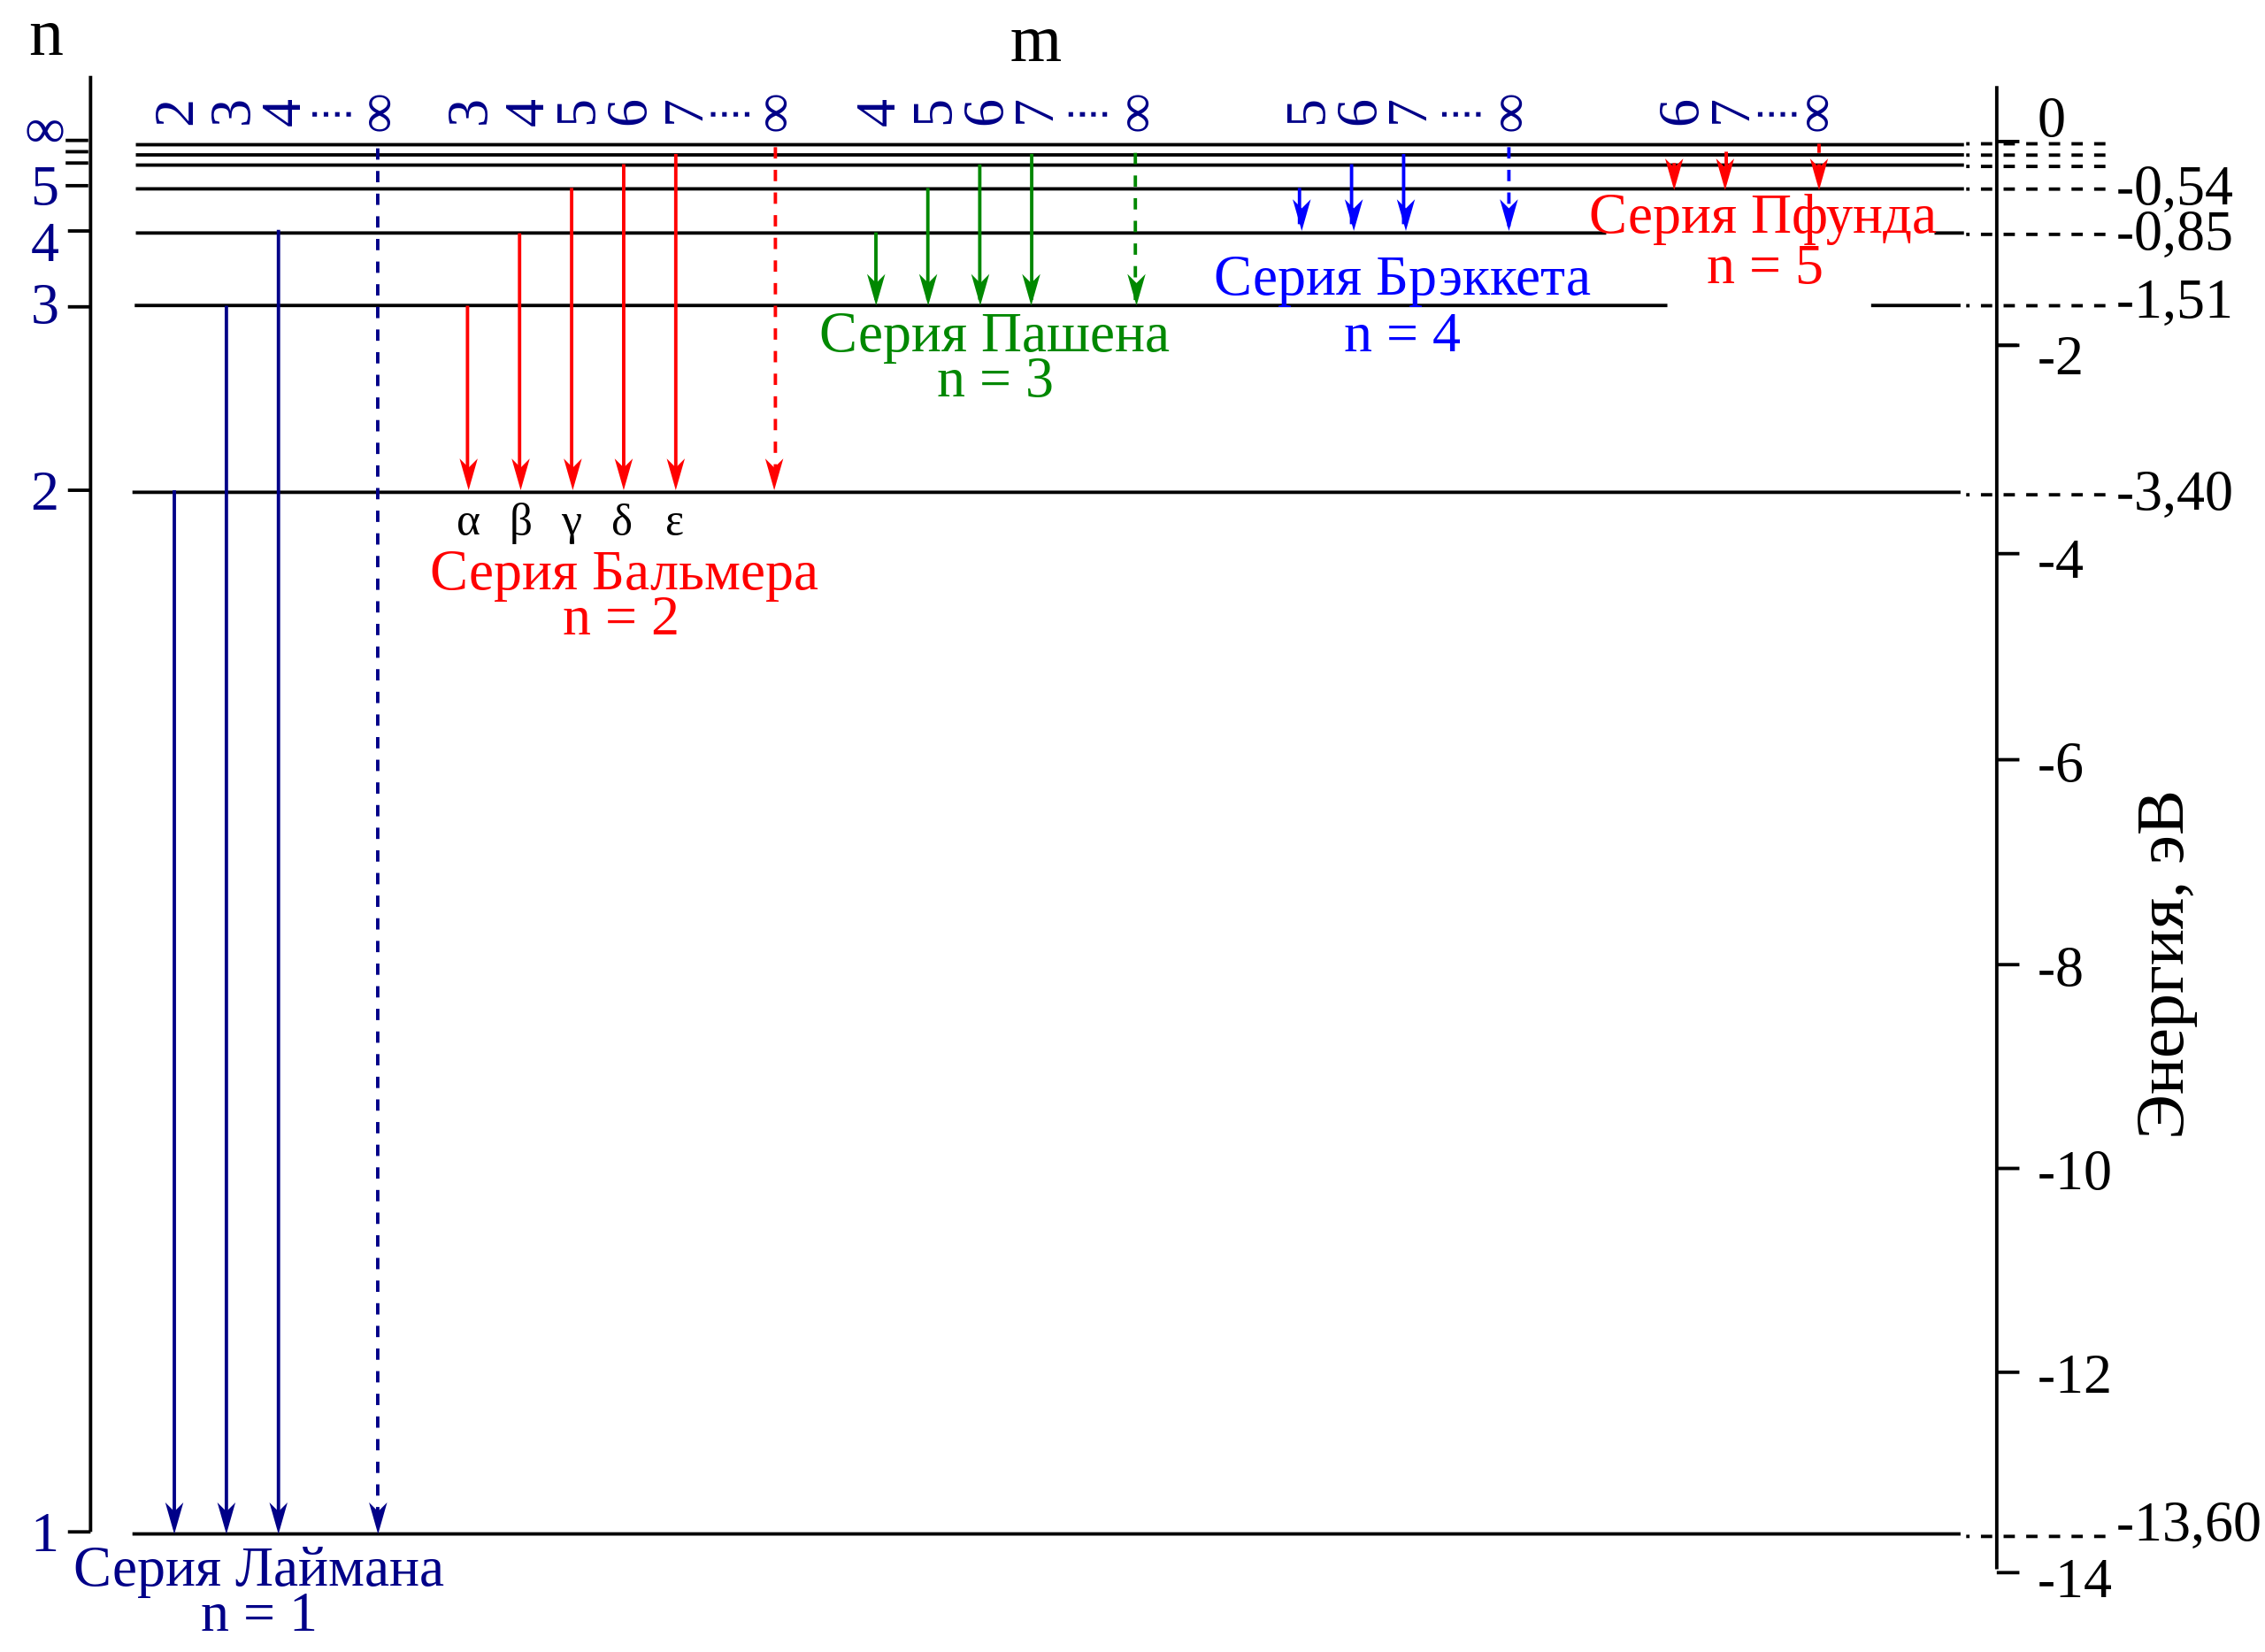
\includegraphics[width=1\textwidth]{Wasserstoff-Termschema-2-ru.svg.png}
    \caption{Спектр водорода}
    \label{fig:H}
\end{figure}
	В данной работе изучается серия Бальмера, линии которой лежат в видимой области. Для серии Бальмера $ n = 2 $. Величина $ m $ для первых четырех линий этой серии принимает значение 3, 4, 5, 6. Эти линии	обозначаются символами $ H_\alpha,\;H_\beta,\;H_\gamma,\;H_\delta $.
	
	Оценим энергии основного и возбужденного состояний водородоподобного атома. Чтобы найти основное состояние квантовой системы, надо минимизировать, с учетом соотношения неопределенностей, полную энергию. Потенциальная энергия электрона равна кулоновской энергии электрона в поле ядра с зарядом $ Z e $. Так как электрон локализован в области размером $ r $, то его импульс $ p \simeq \hbar / r $, и полная энергия определяется выражением
\begin{equation}\label{eq:energy}
		E = \dfrac{-Z e^2}{r}+\dfrac{\hbar^2}{2 m_e r^2}.
\end{equation}
Приняв за нуль производную этого выражения, получим
\begin{equation*}
	r_{\text{Б}} = \dfrac{\hbar^2}{Z m_e e^2}.
\end{equation*}
Это значение радиуса первой орбиты для электрона в поле ядра с зарядом $ Z $ -- боровского радиуса. Подставляя в \eqref{eq:energy} это значение, получим
\begin{equation*}
	E = -R Z^2,
\end{equation*}
\begin{equation}
	R = \dfrac{m_e e^4}{2 \hbar^2}.
\end{equation}
Для возбуждённых состояний значения энергий можно найти аналогично, приняв во внимание, что $ p \simeq n \hbar / r $ из условия, что на длине орбиты укладывается целое число волн де Бройля. Отсюда энергия $ n $-го уровня равна 
\begin{equation*}
	E = \dfrac{-R Z^2}{n^2}.
\end{equation*}

\subsection*{Спектр йода}
В первом приближении энергия молекулы может быть представлена в виде:
\begin{equation}
	E=E_e+E_o+E_r,
\end{equation}
где $E_e$ есть энергия электронных уровней, $E_o$ есть энергия колебательньных уровней, $E_r$ есть энергия вращательных уровней.


\begin{figure}[H]
    \centering
    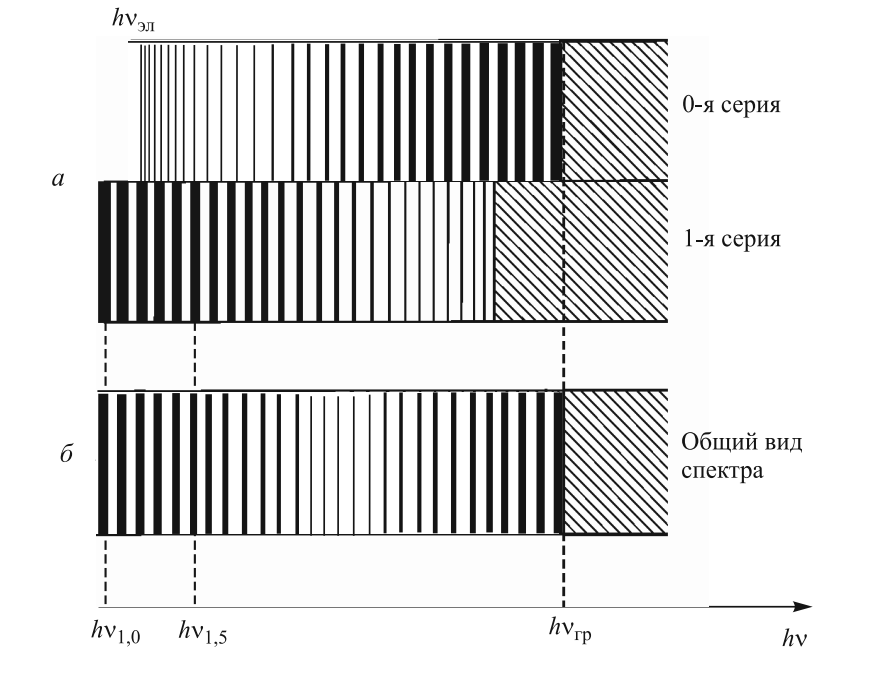
\includegraphics[width=0.5\textwidth]{iod.png}
    \caption{Спектр йода}
    \label{fig:iod}
\end{figure}

В настоящей работе рассматриваются оптические переходы, то есть переходы, связанные с излучением фотонов в видимом диапазоне длин волн. Они соответсвтуют переходам между различными электронными состояниями. При этом также происходят изменения вращательного и колебательного состояний, однако в реальности ввиду малости характерных энергий вращательные переходы ненаблюдаемы.

Более конкретно, изучаются переходы из колебательного состояния с номером $n_1$ освновного электронного уровня с энергией $E_1$ в колебательное состояние с номером $n_2$ на электронный уровень с энергией $E_2$. Энергия таких переходов описывается формулой:
\begin{equation}
	h \nu_{n_1,n_2}=(E_2-E_1)+h\nu_2(n_2+\dfrac{1}{2})-h \nu_1(n_1+\dfrac{1}{2}),
\end{equation}
где $\nu_1$ и $\nu_2$ суть энергии колебательных квантов на электронных уровнях с энергиями $E_1$ и $E_2$.

При достаточно больших квантовых числах $n_1$ и $n_2$ колебательные уровни переходят в непрерывный спектр, что соответствует диссоциации молекулы. Наименьшая энергия, которую нужно сообщить молекуле в нижайшем колебательном состоянии, чтобы она диссоциировала, называется энергией диссоциации.

В данной работе определяются энергии диссоциации на первых двух электронных уровнях.


\section{Экспериментальная установка}
Схема установки представлена на рисунке (\ref{fig:set})

\begin{figure}[H]
    \centering
    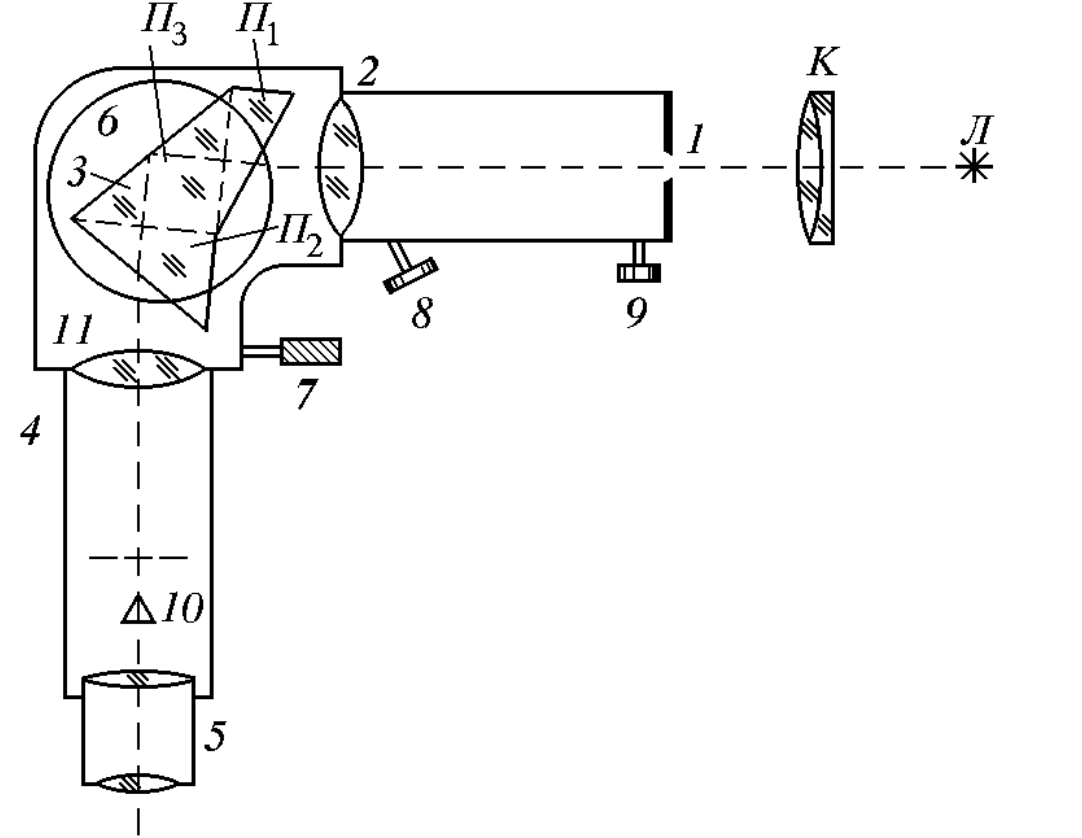
\includegraphics[width=0.7\textwidth]{set.png}
    \caption{Схема установки}
    \label{fig:set}
\end{figure}

Для измерения длин волн спектральных линий в работе используется стеклянный-призменный монохроматор-спектрометр УМ-2 (универсальный монохроматор), предназначенный для спектральных исследований в диапазоне от 0,38 до 1,00 мкм. 

\section{Выполнение работы}
Построим калибровочный график монохроматора по спектрам неона и ртути:

\begin{figure}[H]
    \centering
    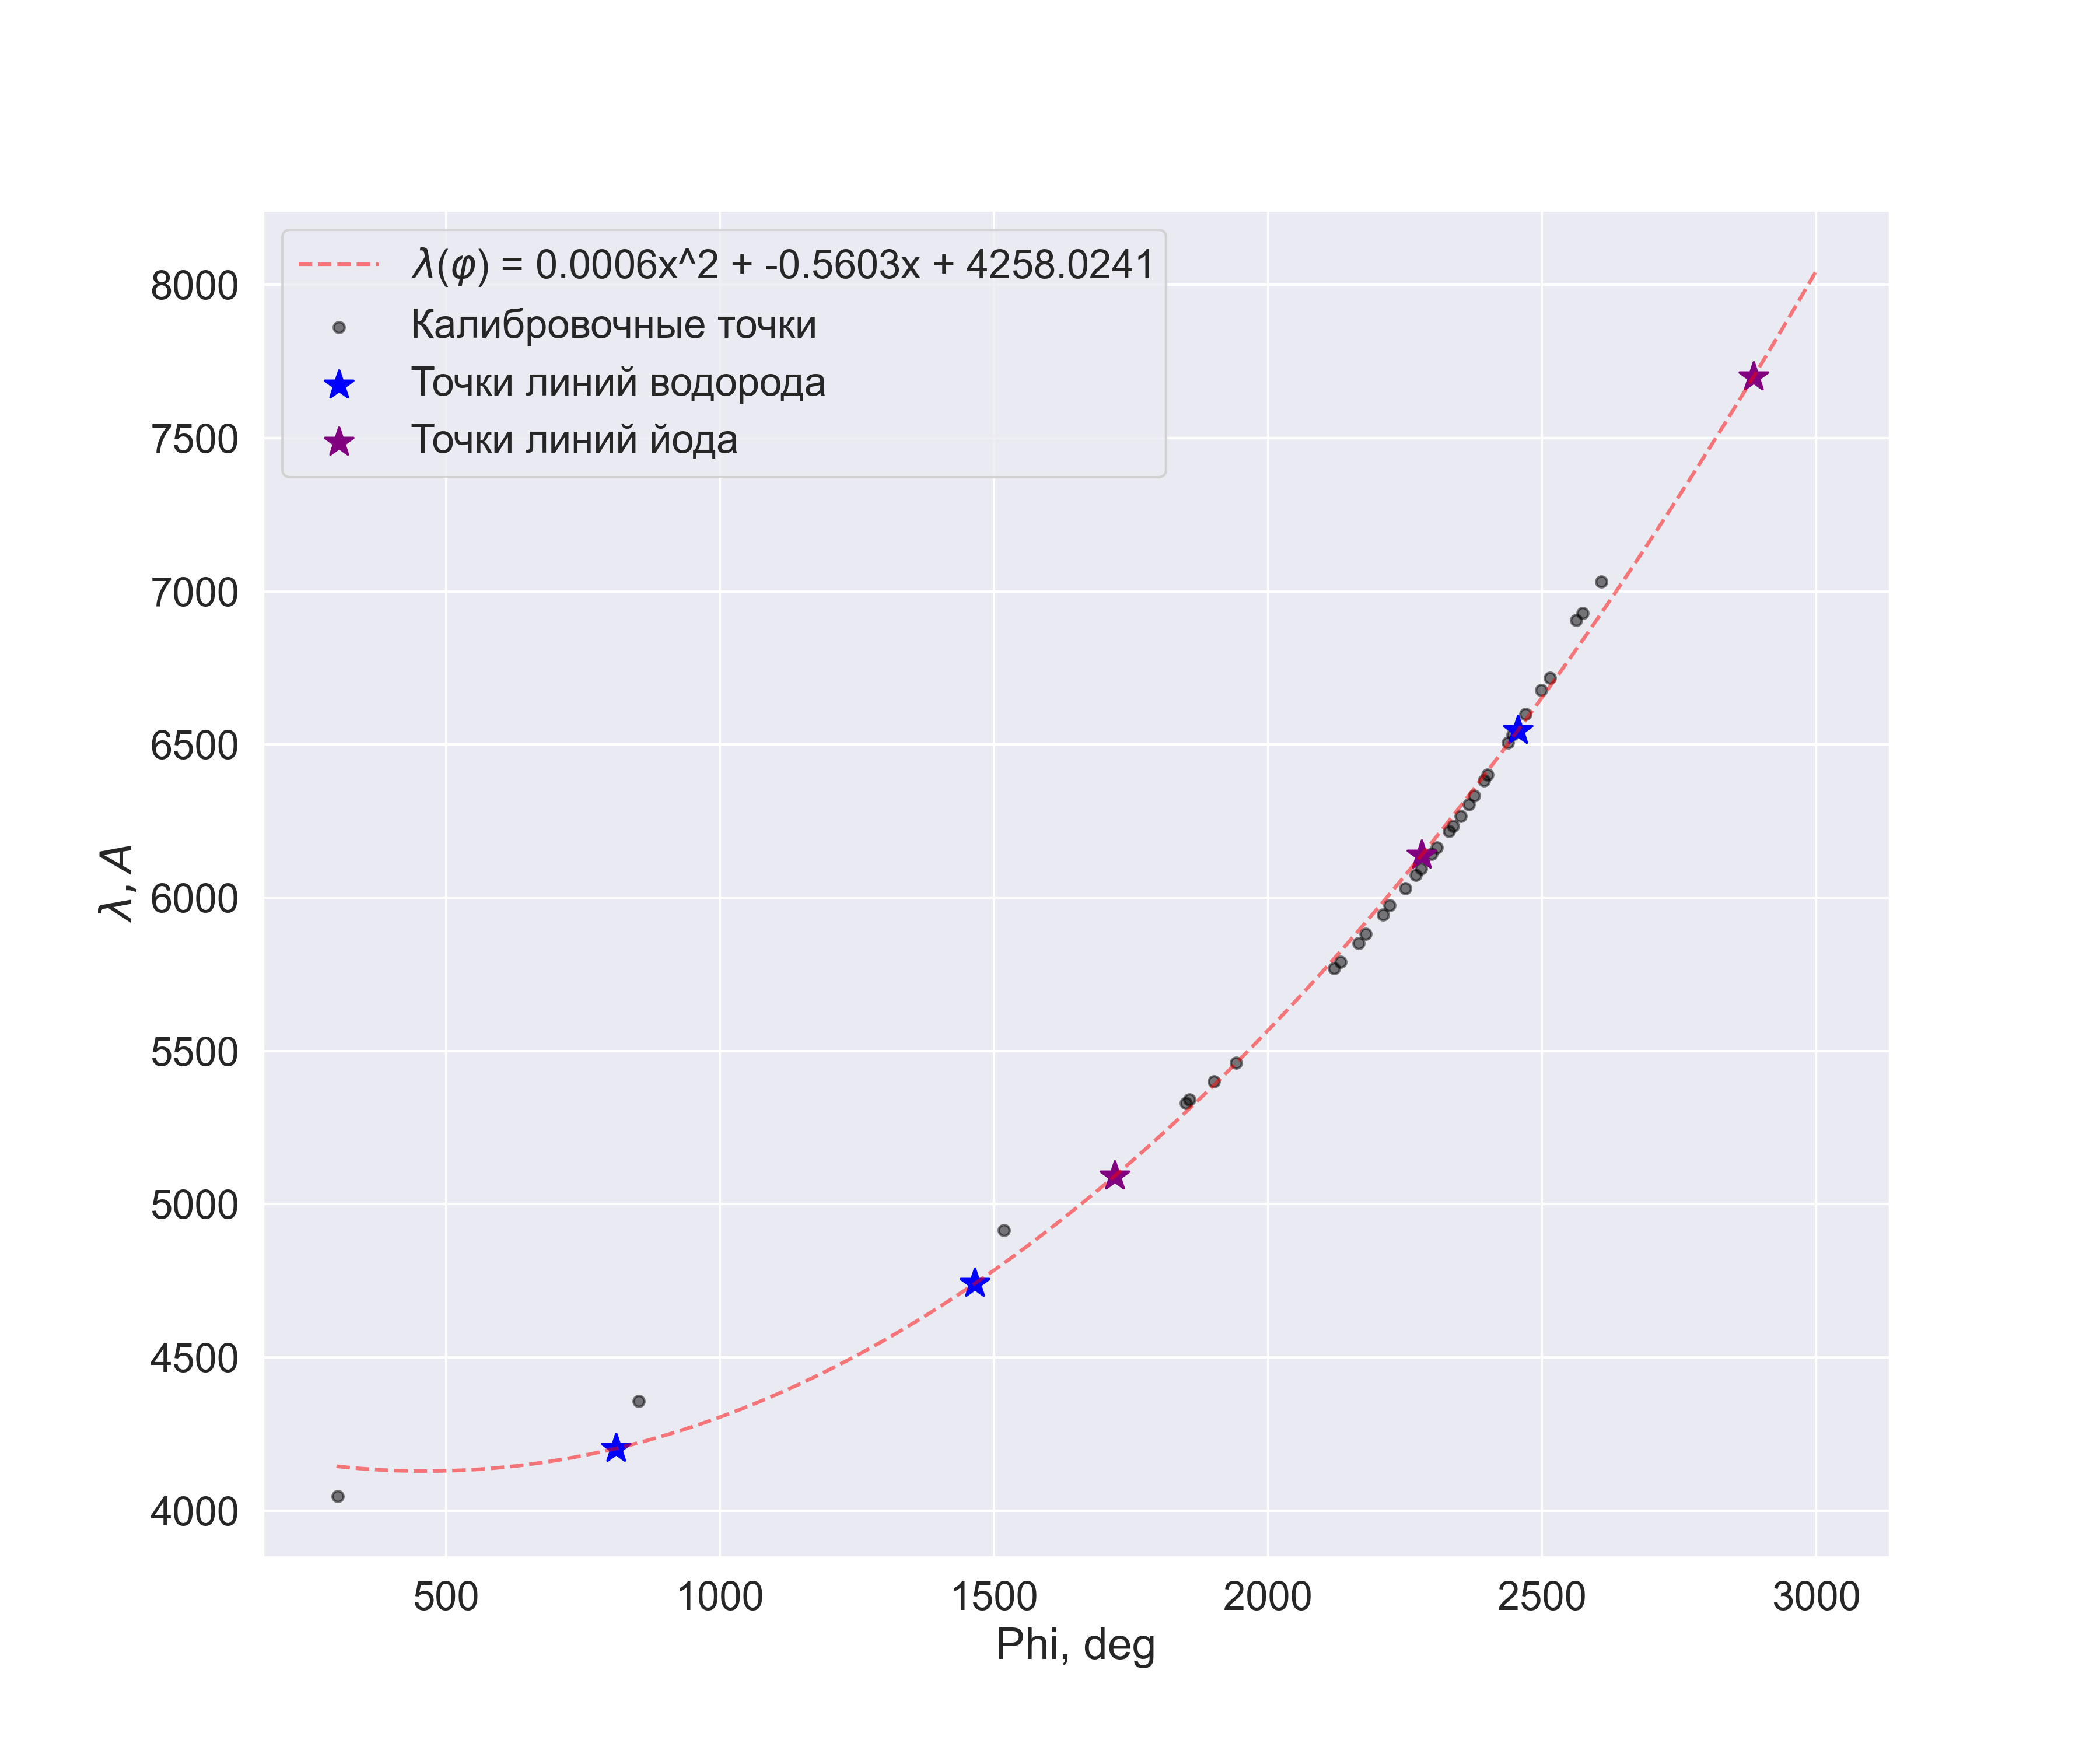
\includegraphics[width=1\textwidth]{plot1.png}
    \caption{Калибровочный график}
    \label{fig:cal}
\end{figure}

По графику найдем длины волн, соответсвтующие серии Бальмера

\begin{table}[H]
	\centering
	\begin{tabular}{|c|c|}
	\hline
			   & $\lambda, \text{нм}$ \\ \hline
	$H_\alpha$ & $655 \pm 10$          \\ \hline
	$H_\beta$  & $474 \pm 7$          \\ \hline
	$H_\gamma$ & $420 \pm 6$         \\ \hline
	\end{tabular}
\end{table}

Для этих значений посчитаем значения констант Ридберга и найдем среднее:

\begin{equation}
	R = 11192754 \pm 1000 \text{ м}^{-1}
\end{equation}

Табличное значение $R_{teor} = 10973731 \text{ м}^{-1}$

\section{Выводы}
В ходе работы был изучен спектр атома водорода, получена константа Ридберга. Ее значение совпало с теоретическим. В работе можно было наблюдать линии альфа, бета и гамма.
\end{document}